\documentclass{beamer}

\usefonttheme{professionalfonts} % using non standard fonts for beamer
\usefonttheme{serif} % default family is serif

\usepackage{hyperref}

%\usepackage{minted}

\usepackage{animate}

\usepackage{graphicx}

\def\Put(#1,#2)#3{\leavevmode\makebox(0,0){\put(#1,#2){#3}}}

\usepackage{color}

\usepackage{tikz}

\usepackage{amssymb}

\usepackage{enumerate}


\newcommand\blfootnote[1]{%

  \begingroup

  \renewcommand\thefootnote{}\footnote{#1}%

  \addtocounter{footnote}{-1}%

  \endgroup

}

\makeatletter

%%%%%%%%%%%%%%%%%%%%%%%%%%%%%% Textclass specific LaTeX commands.

 % this default might be overridden by plain title style

 \newcommand\makebeamertitle{\frame{\maketitle}}%

 % (ERT) argument for the TOC

 \AtBeginDocument{%

   \let\origtableofcontents=\tableofcontents

   \def\tableofcontents{\@ifnextchar[{\origtableofcontents}{\gobbletableofcontents}}

   \def\gobbletableofcontents#1{\origtableofcontents}

 }

%%%%%%%%%%%%%%%%%%%%%%%%%%%%%% User specified LaTeX commands.

\usetheme{Malmoe}

% or ...

\useoutertheme{infolines}

\addtobeamertemplate{headline}{}{\vskip2pt}



\setbeamercovered{transparent}

% or whatever (possibly just delete it)

\makeatother

\begin{document}
\title[PFLOCK report]{PFLOCK Report}
\author[AC]{Andres Calderon}
\institute[Summer'19]{University of California, Riverside}
\makebeamertitle
\newif\iflattersubsect

\AtBeginSection[] {
    \begin{frame}<beamer>
    \frametitle{Outline} 
    \tableofcontents[currentsection]  
    \end{frame}
    \lattersubsectfalse
}

\AtBeginSubsection[] {
    \begin{frame}<beamer>
    \frametitle{Outline} 
    \tableofcontents[currentsubsection]  
    \end{frame}
}

\begin{frame}{Testing MF Algorithm (Uniform dataset)}
    \begin{itemize}
        \item Test MF algorithm in a uniform distributed dataset:
        \begin{itemize}
            \item 100K points distributed in the same LA region.
            \item Using grid partitioning.         
            \item $\varepsilon = 25$, $\mu = 5$.
        \end{itemize}
    \end{itemize}
    \centering
    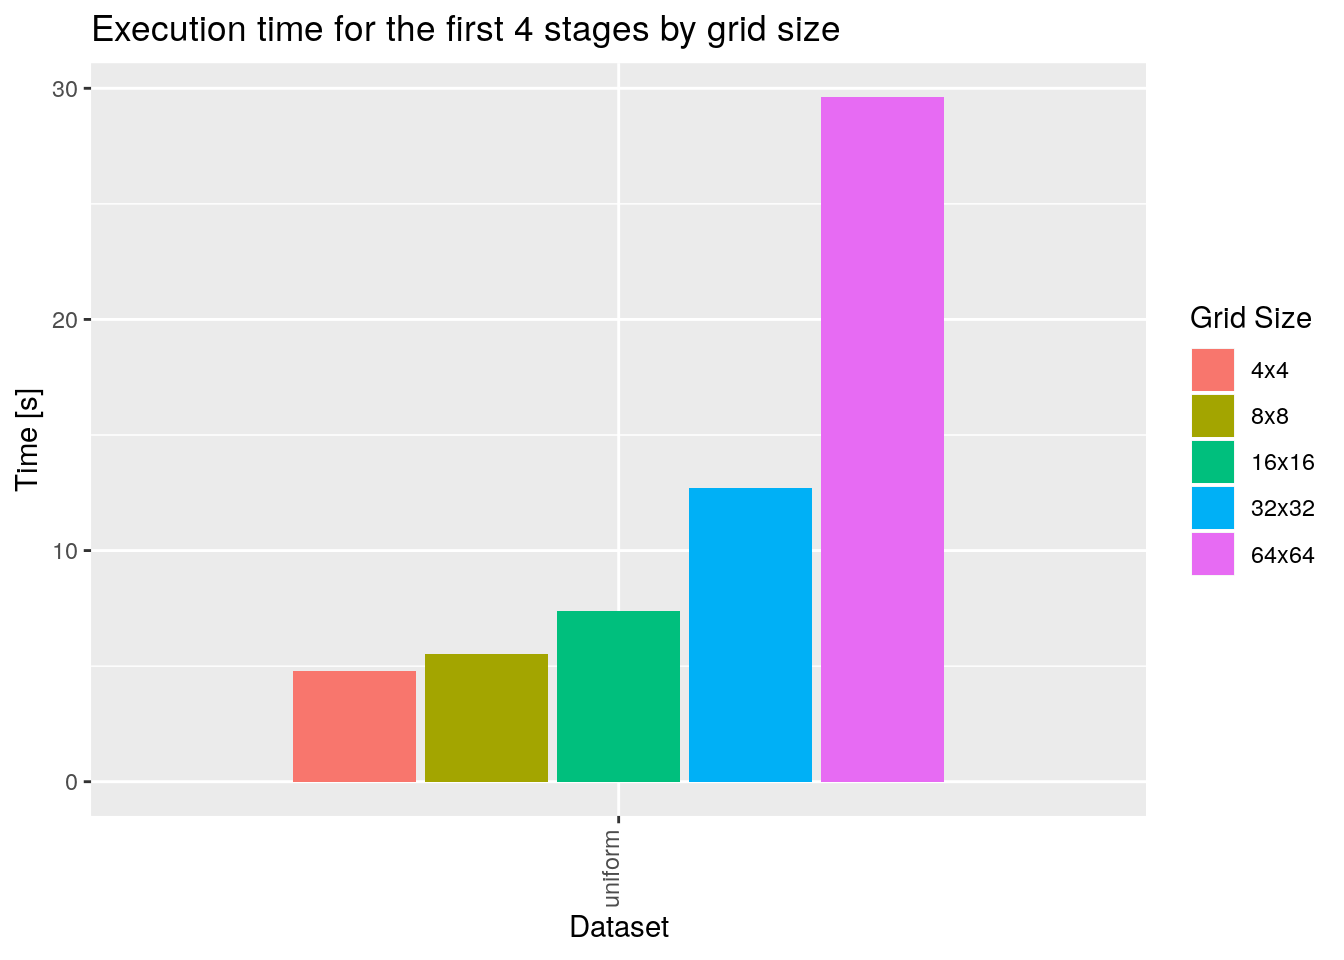
\includegraphics[width=0.65\textwidth]{figures/01_uniform.png}
\end{frame}

\begin{frame}{Testing MF Algorithm (Uniform dataset)}
    \begin{itemize}
        \item Break down uniform distributed dataset by stage (first 4 stages for now)
    \end{itemize}
    \centering
    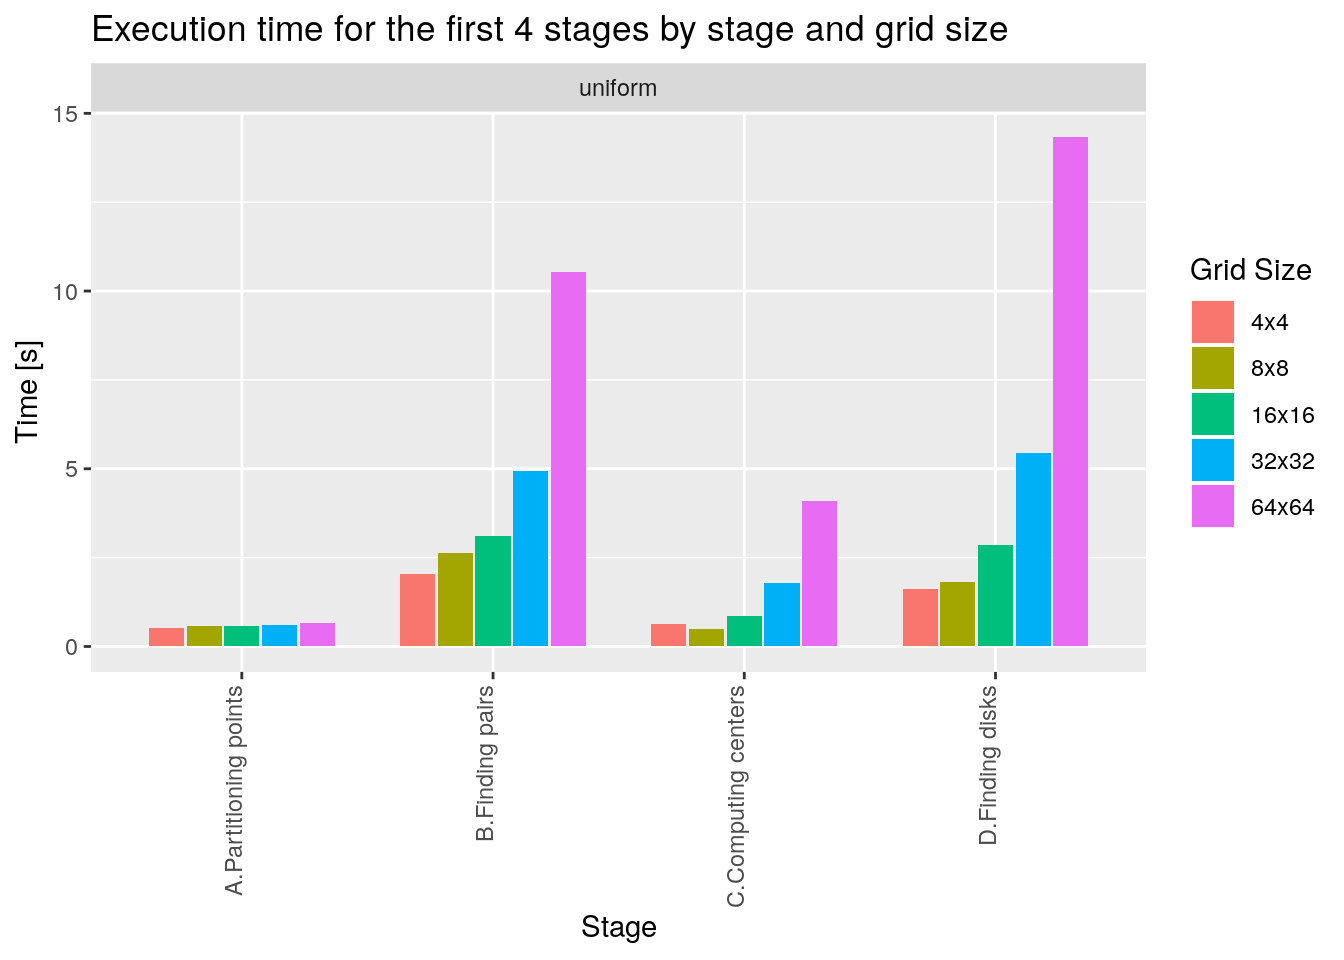
\includegraphics[width=0.7\textwidth]{figures/02_uniformByStages.png}
\end{frame}

\begin{frame}{Testing MF Algorithm (Uniform dataset)}
    \begin{itemize}
        \item Indeed, in uniform dataset is possible to reach larger epsilon values ($\mu=5$):
    \end{itemize}
    \centering
    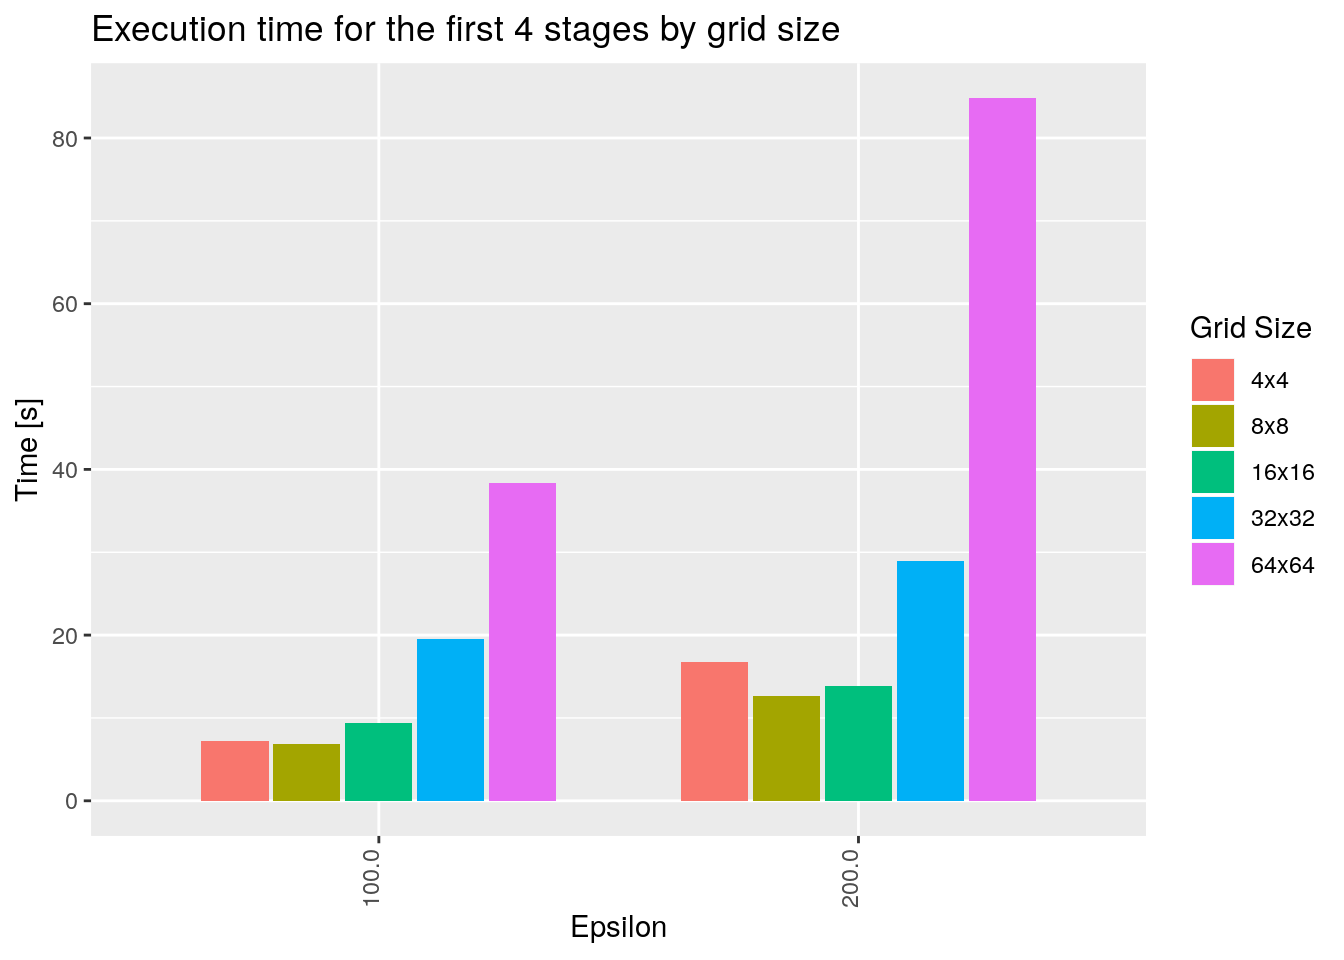
\includegraphics[width=0.7\textwidth]{figures/03_uniformLarge.png}
\end{frame}

\begin{frame}{Testing MF Algorithm (Uniform dataset)}
    \begin{itemize}
        \item Indeed, in uniform dataset is possible to reach larger epsilon values ($\mu=5$):
    \end{itemize}
    \centering
    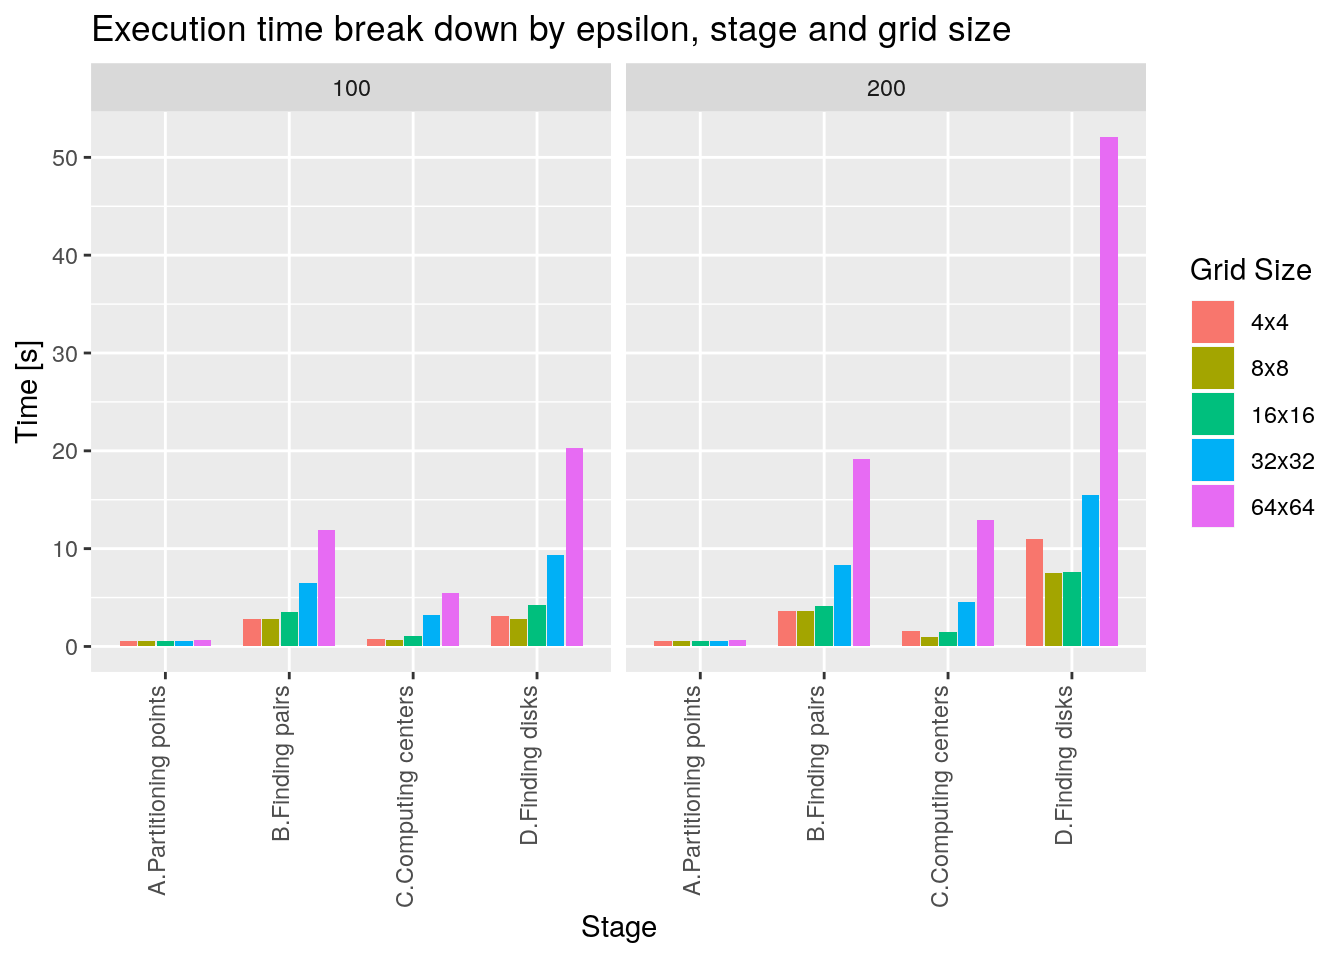
\includegraphics[width=0.7\textwidth]{figures/04_uniformLargeByStages.png}
\end{frame}

\begin{frame}{What to do with skew datasets}
    \begin{itemize}
        \item That is promising but uniform datasets are quite unrealistic.
        \item Also, MF should be able to deal with some kind of skew data.
        \item So, let's explore a Quadtree partitioning:  a coarse quadtree for the first 4 stages and a finer one for the last 2.
    \end{itemize}
\end{frame}

\begin{frame}{Quadtree in GeoSpark}
    \begin{itemize}
        \item Hacking a bit the GeoSpark Quadtree partitioner to have access to the main parameters:
        \begin{itemize}
            \item \texttt{MaxLevel}: Maximum level of the tree.  It controls how deep will be the tree.  Keeping this value high will allow finer partitioning.
            \item \texttt{MaxEntries}: Maximum number of entries (capacity) of each cell.  If a cell reaches the maximum capacity it will split.
        \end{itemize}
        \item So, keeping a relatively high value of \texttt{MaxLevel}, variying the value of \texttt{MaxEntries} will control the number of partitions in the Quadtree.
    \end{itemize}
\end{frame}

\begin{frame}{Testing MF Algorithm (Quadtree partitioning)}
    \begin{itemize}
        \item Finding the \texttt{MaxEntries} optimal value for the first 4 stages.
        \item Testing LA\_50K and LA\_100K datasets. 
    \end{itemize}
    \centering
    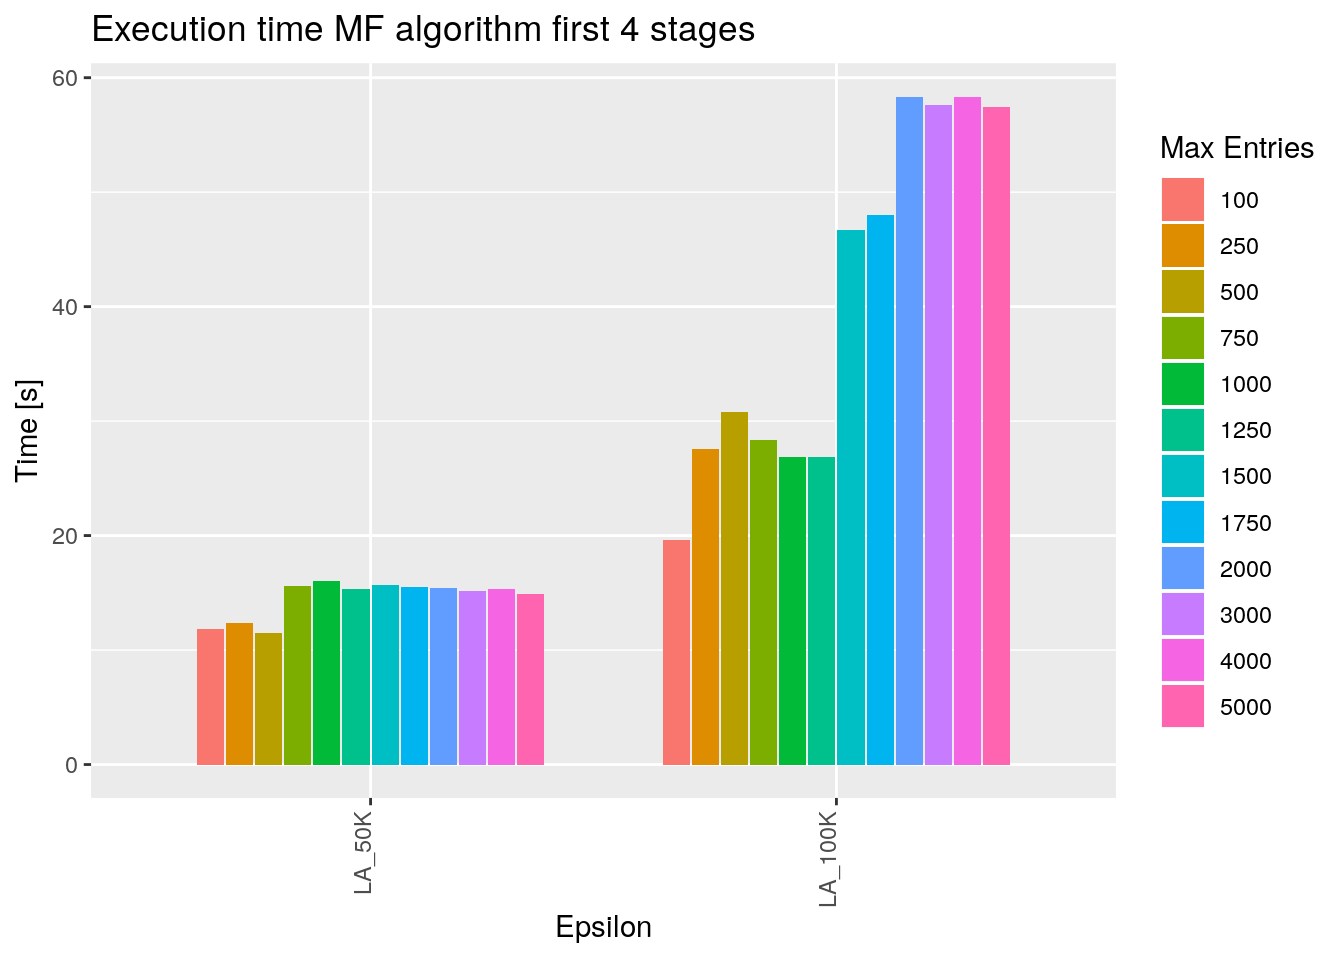
\includegraphics[width=0.8\textwidth]{figures/05_QuadtreeFirstStages.png}
\end{frame}

\begin{frame}{Testing MF Algorithm (Quadtree partitioning)}
    \begin{itemize}
        \item Finding the \texttt{MaxEntries} optimal value for the last 2 stages.
        \item Testing LA\_50K. Using \texttt{MaxEntries = 500} for the first quadtree.
        \item $\varepsilon = 10$, $\mu = 5$.
    \end{itemize}
    \centering
    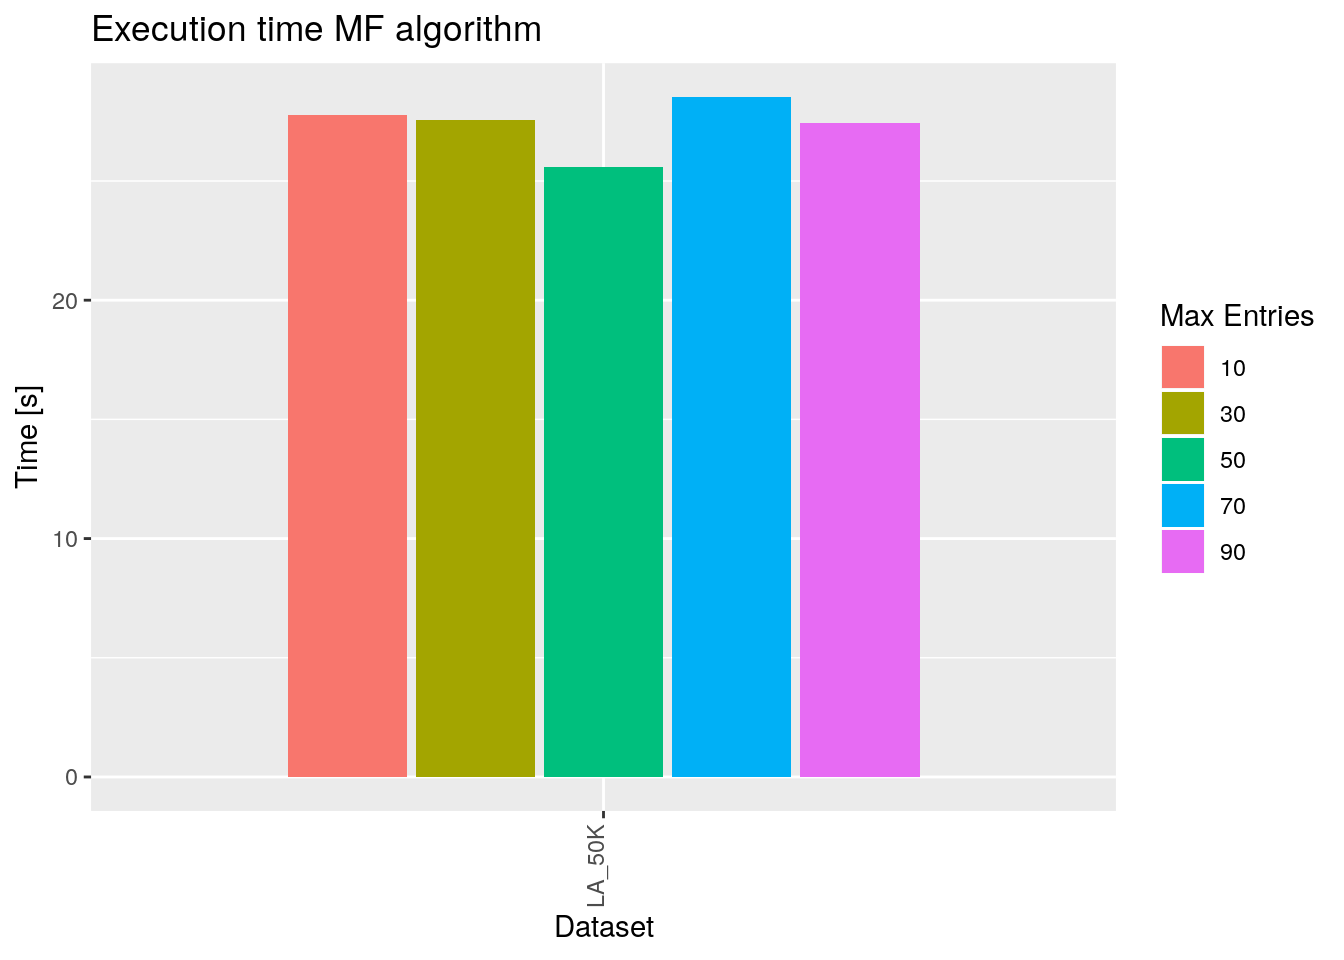
\includegraphics[width=0.65\textwidth]{figures/06_Quadtree2LA_50K.png}
\end{frame}

\begin{frame}{Testing MF Algorithm (Quadtree partitioning)}
    \begin{itemize}
        \item Finding the MaxEntries optimal value for the last 2 stages.
        \item Testing LA\_100K. Using \texttt{MaxEntries = 100} for the first quadtree.
        \item $\varepsilon = 7$, $\mu = 5$.
    \end{itemize}
    \centering
    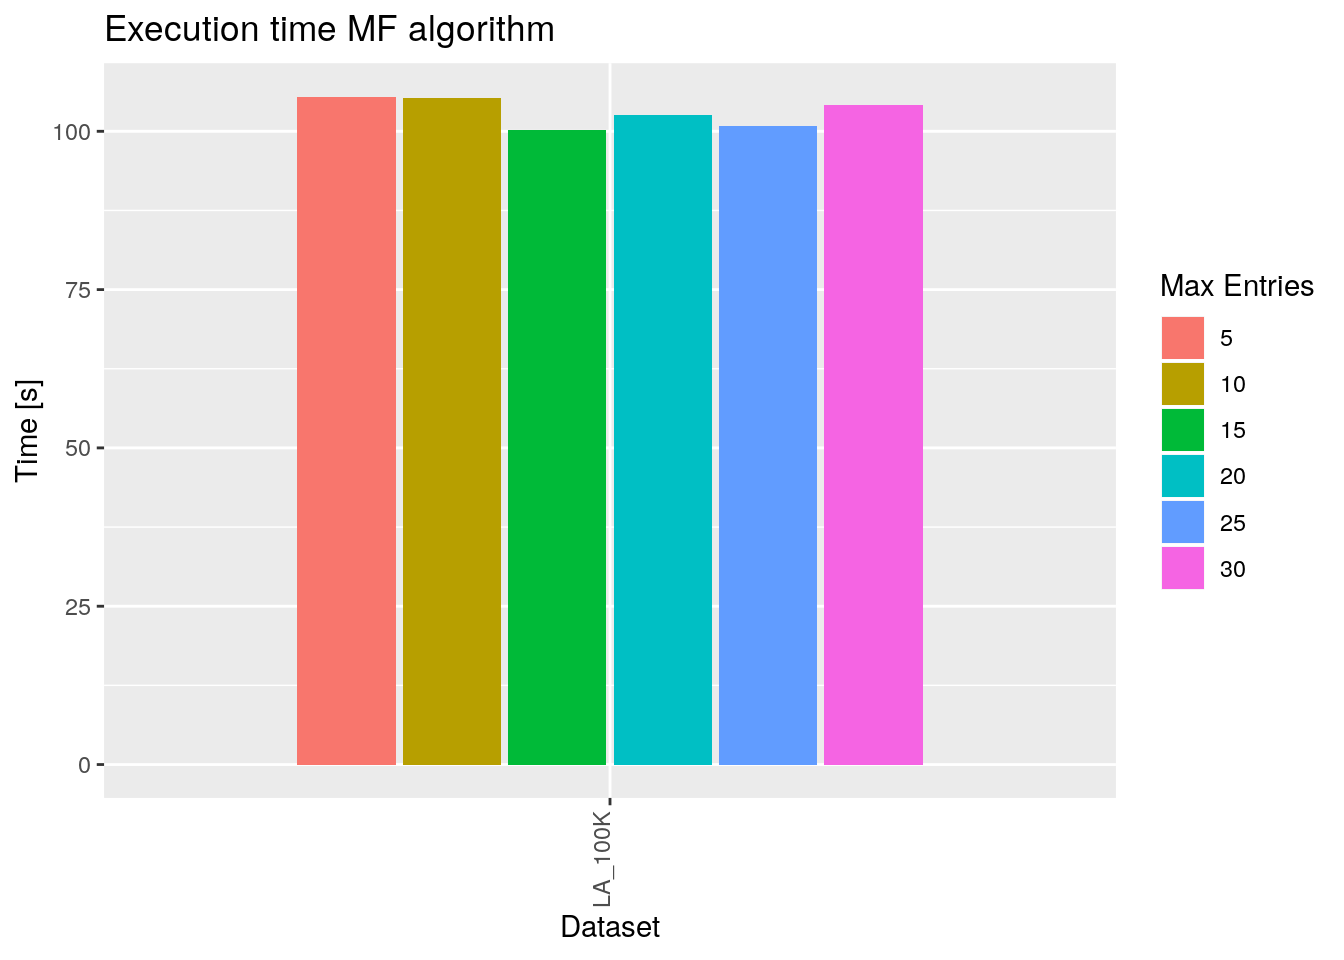
\includegraphics[width=0.65\textwidth]{figures/07_Quadtree2LA_100K2.png}
\end{frame}

\begin{frame}{[Bonus] MF Algorithm (Uniform dataset + Quadtree partitioning)}
    \begin{itemize}
        \item Using first quadtree \texttt{MaxEntries = 1000}.
        \item $\varepsilon = 100$, $\mu = 5$.        
    \end{itemize}
    \centering
    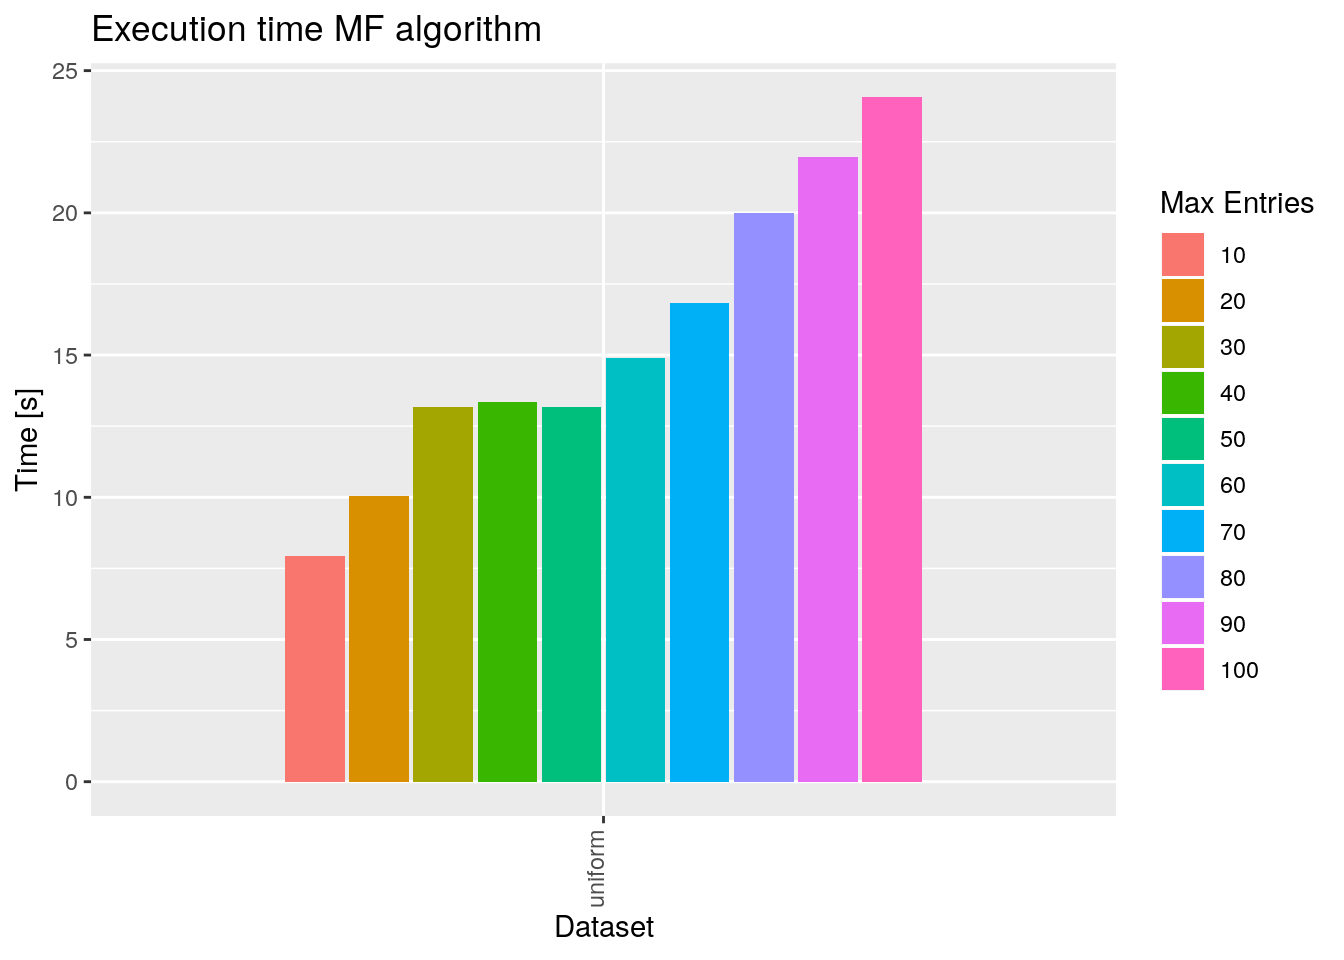
\includegraphics[width=0.65\textwidth]{figures/08_Quadtree2uniform.png}
\end{frame}
\end{document}
